\documentclass[thesis.tex]{subfiles}
\begin{document}

\chapter{Einführung}
\label{chap:introduction}

\begin{figure}[h!]
\centering
\begin{subfigure}{.32\textwidth}
    \centering
    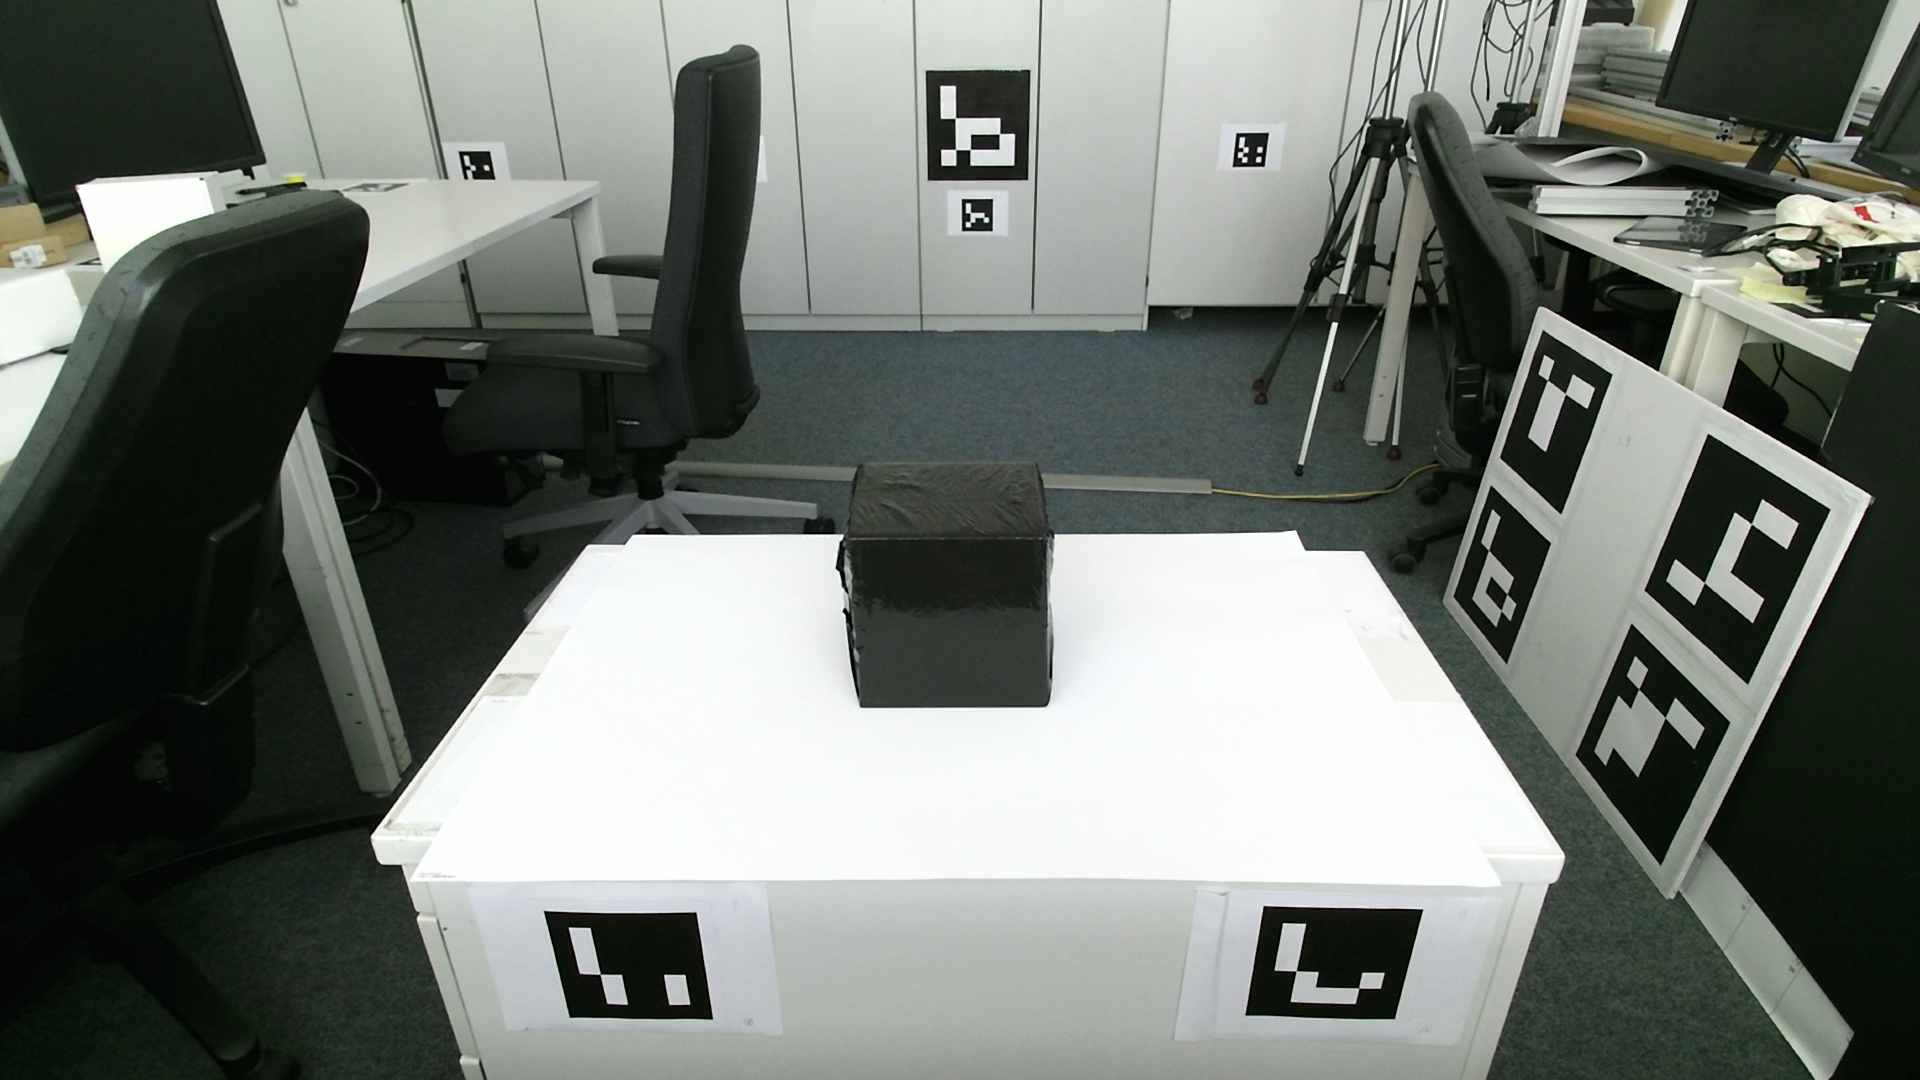
\includegraphics[width=.95\linewidth]{Kinect_introduction/rgb}
    \caption{Farbbild}
\end{subfigure}%
\begin{subfigure}{.32\textwidth}
    \centering
    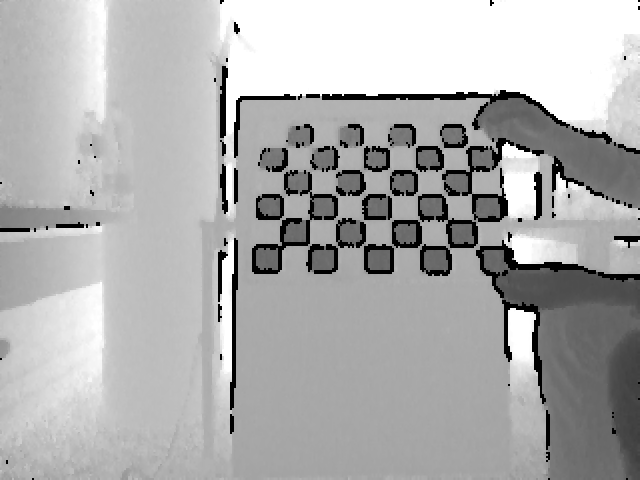
\includegraphics[width=.95\linewidth]{Kinect_introduction/ir}
    \caption{Infrarotbild}
\end{subfigure}
\begin{subfigure}{.32\textwidth}
    \centering
    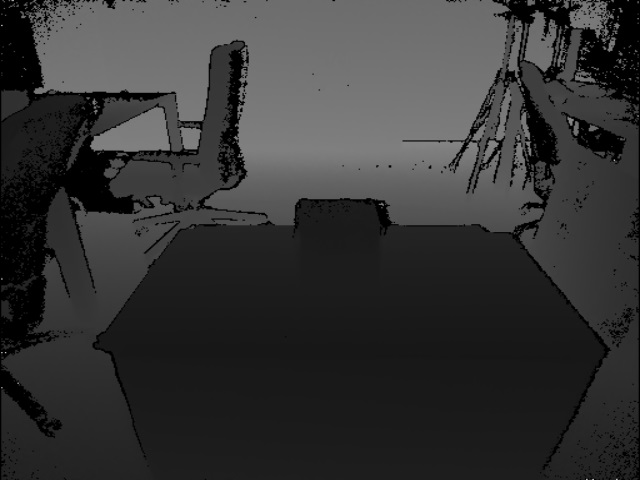
\includegraphics[width=.95\linewidth]{Kinect_introduction/depth}
    \caption{Tiefenbild}
\end{subfigure}
\caption{Die einzelnen Kamera Streams, die von der Microsoft Kinect v2 geliefert werden.}
\label{fig:introduction_picture}
\end{figure}

\section{Einleitung}

Time-of-Flight Kameras haben in der Wissenschaft besonders nach der Veröffentlichung der Kinect v2 deutlich an Bedeutung gewonnen, da diese den bisherigen Technologien in Geschwindigkeit und Genauigkeit auch auf große Entfernungen überlegen waren und zudem durch den niedrigen Preis für Endnutzer und die Forschung interessant wurden. So fanden die Tiefensensoren, die ursprünglich für Unterhaltungsbereich konzipiert wurden, auf Gebieten wie der Robotik und Medizin Anwendung \cite{bib:Meister2013}\cite{bib:Hertzberg2014}\cite{bib:Villena-Martinez2017}. Auch in der Logistik gewinnen preiswerte und robuste Kamera Systeme an Bedeutung für den Endnutzer, da diese zur flächendeckenden Überwachung eingesetzt werden und zuverlässig korrekte Werte liefern sollten, wobei sie um anderen günstig in der Anschaffung sind. Bei Time-of-Flight Kameras handelt es sich um Tiefensensoren, die mittels kurzer Lichtpulse die Entfernung von Objekten messen, indem die Flugzeit des Lichts geschätzt wird. Dabei kommt es nicht nur zu direkten Reflexionen, sondern auch zu indirekten Reflexionen an Oberflächen. Daher ist es wichtig für die Simulation eben diese indirekte Beleuchtung zu berücksichtigen, da sich diese auf die geschätzten Distanzen im Tiefenbild auswirkt. In \autoref{fig:introduction_picture} wird veranschaulicht, welche Bilder das Microsoft Kinect v2 Kamerasystem aufnimmt. Dabei handelt es sich um ein RGB-D Kamerasystem, das sowohl das Abgreifen von Farbbildern, als auch das von Tiefenbildern ermöglicht.

Aus der Literatur bekannte Simulationen von Time-of-Flight Sensoren lassen sich in zwei Kategorien einteilen: die interaktiven Simulationen, die es dem Nutzer ermöglichen Eingaben zu tätigen, die direkte Auswirkungen auf die Szene haben und durch die so beispielsweise Anpassungen an der Ausrichtung der Kamera durchgeführt werden können und die nicht-interaktiven Simulationen, in denen die Einstellungen im Vorfeld vorgenommen werden und bei denen die Berechnung einen Zeitraum von einigen Minuten in Anspruch nimmt. Um als interaktiv bezeichnet werden zu können, sollte eine Anwendung das Bild innerhalb von 50 ms generiert haben oder in dem Zeitraum ein Zwischenergebnis liefern können, das dem Nutzer ein Feedback über das mögliche Endresultat gibt \cite{bib:Claypool-Damaa2006}. Die Time-of-Flight Kameras mit der höchsten Anzahl an Bildern pro Sekunde, die in dieser Arbeit genutzt werden, liefern die Bilder innerhalb von 33 ms, weshalb diese Zeitspanne als Grenze für eine Echtzeitsimulation betrachtet wird.

\section{Motivation und Herausforderungen}

\begin{figure}[h!]
\centering
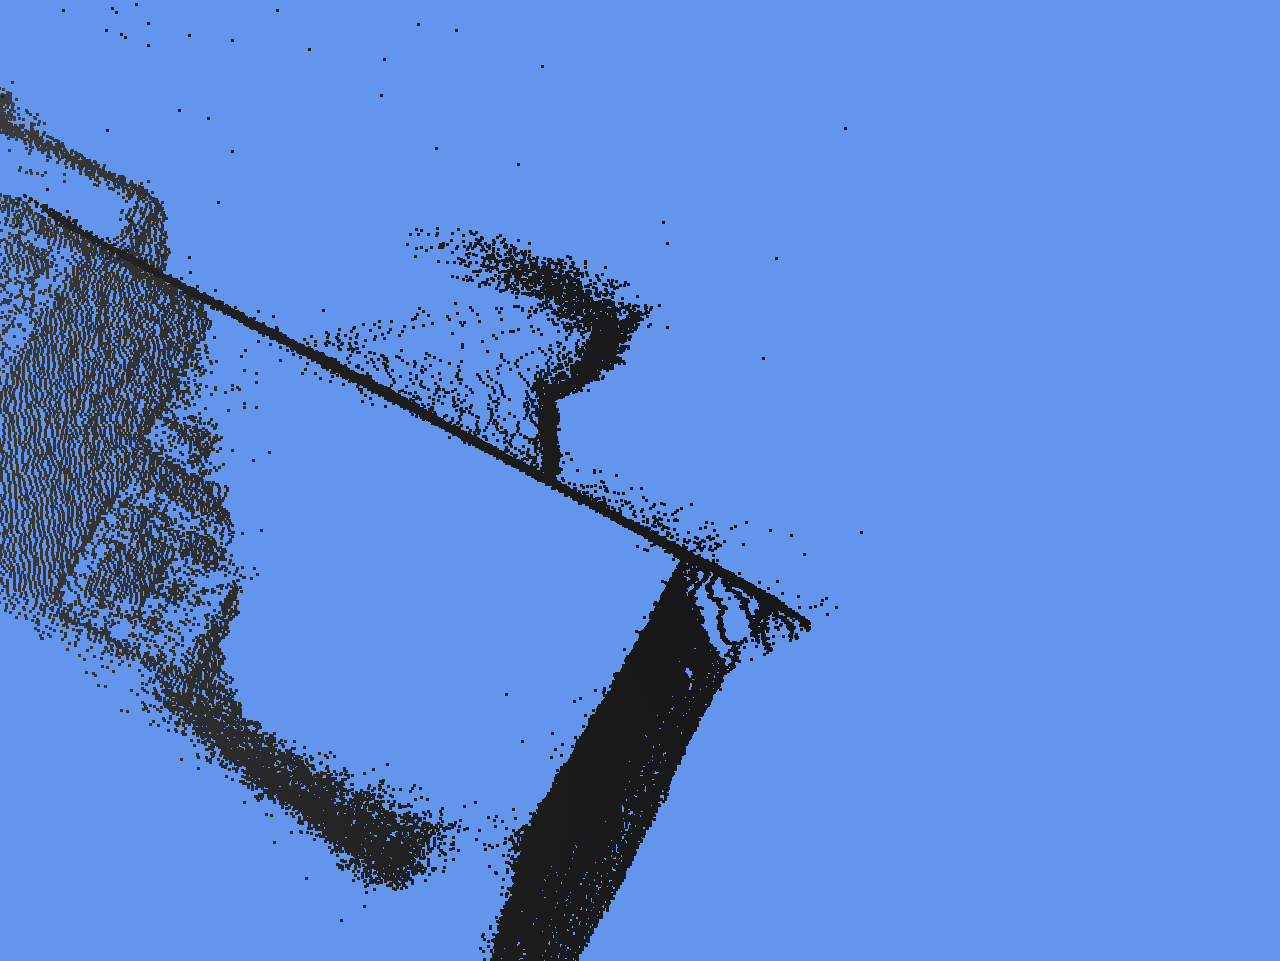
\includegraphics[width=.50\linewidth]{Kinect_introduction/distortion}
\caption{Die Punktewolke, die aus dem vorher gezeigten Tiefenbild erstellt wurde, auf dem der Einfluss durch die indirekte Beleuchtung auf den Kubus zu sehen ist.}
\label{fig:motivation_picture}
\end{figure}

Wie bereits erwähnt sind die Tiefenbilder von Time-of-Flight Kameras Effekten durch indirekte Beleuchtung ausgesetzt, was in \autoref{fig:motivation_picture} veranschaulicht wird. Diese zeigt dabei dieselbe Szene wie \autoref{fig:introduction_picture} aus einer anderen Perspektive, von der aus die Verzerrungen am Kubus zu erkennen sind, die durch die indirekte Beleuchtung der Oberfläche verursacht werden. Dies führt besonders in jenen Anwendungen zu Problemen, die diese Tiefenwerte zur Weiterverarbeitung verwenden, um Informationen über die aufgenommene Szene zu erhalten. Da diese Fehler stark Blickwinkelabhängig sind, führen sie dazu, dass Daten fehlerhaft ausgewertet werden und z. B. autonome Maschinen falsch auf den gelieferten Input reagieren. Während der Entwicklung von autonomen Systemen und in der Robotik wird häufig in simulierten Umgebungen gearbeitet, da fehlerhafte Implementierungen die Zerstörung von Geräten wie Drohnen oder autonomen Fahrzeugen zur Folge haben könnten, weshalb eine akkurate Simulation der genutzten Time-of-Flight Kameras wichtig ist \cite{bib:Meister2013}. Da Time-of-Flight Kameras beispielsweise auch in der Mensch-Maschine Interaktion verwendet werden, könnte eine Reaktion auf einen fehlerhaften Input folgenschwere Konsequenzen nach sich ziehen, falls diese Artefakte nicht bereits während der Entwicklung berücksichtigt wurden. Einige wissenschaftliche Arbeiten beschäftigen sich außerdem mit der Korrektur dieser Artefakte, die durch Time-of-Flight Kamerasystemen verursacht werden \cite{bib:Su2018}\cite{bib:Mure-Dubois2007}\cite{bib:Mure-Dubois2009}\cite{bib:Freedman2014}. Die Simulation bietet auch hier Vorteile, da Referenzwerte zur Verfügung stehen, die beispielswiese zum Trainieren von neuronalen Netzen verwendet werden können \cite{bib:Su2018}. Zusätzlich bietet eine Simulation im Gegensatz zu einer echten Aufnahme die Möglichkeit Artefakte isoliert zu betrachten und andere Störfaktoren zu entfernen, während bei echten Aufnahmen entweder keine oder ungenaue Referenzwerte zur Verfügung stehen und Artefakte nicht ausgeblendet werden können \cite{bib:Nair2013}.

Bei der Simulation von Time-of-Flight Kameras wird man vor Herausforderungen gestellt, die bisweilen nicht ohne zeitintensive Berechnungen bewältigt werden können. So erfordert die korrekte Simulation der Lichtausbreitung des Infrarotimpulses die Berechnung mehrerer Reflexionen an Oberflächen, bevor das Licht zum Sensor gelangt. Außerdem führen Reflexionen innerhalb der Linse und Beugung an der Blende zu weiteren Artefakten, die sich auf die Korrektheit der Tiefenwerte auswirkt, die in einer Simulation berücksichtig werden müssen. Darüber hinaus führt die Bewegung der Kamera und die Bewegung von Objekten im Bild während der Aufnahme zu Motion Blur Artefakten, die sich je nach Chip-Architektur des Sensors anders gestalten können. Mit diesem Problem haben sich bereits Forschungsarbeiten beschäftigt \cite{bib:Lambers2015}.

Durch die zeitintensive Berechnung in den eben genannten Fällen greifen themenverwandte Untersuchungen entweder auf vorberechnete Lichtsimulationen zurück, die ausschließlich den Einsatz in statischen Szenen erlauben, oder sie verzichten auf die Simulation der Artefakte und konzentrieren sich auf einzelne Teilaspekte, wie die Simulation der Bewegungsunschärfe, während der Einfluss indirekter Beleuchtung ignoriert wird \cite{bib:Keller2015}\cite{bib:Lambers2015}.

\section{Ziele der Arbeit}

Diese Arbeit verfolgt das Ziel einer phyikalisch plausiblen interaktiven Simulation von Time-of-Flight Sensoren unter Berücksichtigung möglichst vieler Artefakte. Zu diesem Zweck werden Algorithmen eingesetzt, die auf der Grafikkarte parallelisiert werden können. 

Da es sich hierbei um eine zeitlich begrenzte Arbeit handelt, unterliegt diese einigen Limitationen, weshalb nicht alle Effekte simuliert werden können. Beispielsweise wird auf die Simulation der Bewegungsunschärfe verzichtet, da diese eine umfangreiche Untersuchung voraussetzt, was den Rahmen der Arbeit sprengen würde. Allerdings wird die Korrektheit der Berechnung der Reflexionen an Oberflächen priorisiert, sodass die Reduktion der Berechnungszeit nur zweitrangige Priorität hat. Dabei wird vollständig auf Vorberechnungen innerhalb der Simulation verzichtet und auf die dynamische Simulation der Szene Wert gelegt, damit auf jede mögliche Konfigurations- und Positionsänderung reagiert werden kann. Die Simulation soll dabei größtenteils auf der GPU stattfinden um eine serielle Abarbeitung auf der CPU zu vermeiden, die auf der GPU parallel durchgeführt werden könnte.

Außerdem soll die Simulation auch unabhängig von der gewählten Szene funktionieren und sowohl für enge Räume als auch für große Hallen und offene Gelände unter dem Einfluss der Sonneneinstrahlung oder künstlicher Beleuchtung ensprechend plausible Tiefenwerte liefern können.

\section{Grober Umriss der Arbeit}

In den folgenden Kapiteln werden zunächst theoretische Grundlagen besprochen, die den Untersuchungsgegenstand der Arbeit nachvollziehbar machen. Im darauf folgenden \autoref{chap:analysis} werden die Time-of-Flight Kameras, die zur Referenz genutzt werden, im Detail analysiert. Aus der Literatur bekannte Artefakte werden reproduziert und isoliert betrachtet.

Anschließend wird in \autoref{chap:simulation} die Implementierung der Simulation erläutert und die Ergebnisse in \autoref{chap:evaluation} evaluiert und mit der Kinect v2 verglichen. \autoref{chap:conclusion} fasst die Arbeit abschließend zusammen und gibt einen Ausblick auf mögliche zukünftige Arbeiten, die auf den Ergebnissen dieser Arbeit aufbauen könnten.

\subfilebib % Makes bibliography available when compiling as subfile
\end{document}
